\chapter{CRONOGRAMA}
\label{cap:cronograma}

A Figura~\ref{fig51} apresenta o cronograma previsto para realização das atividades. As colunas representam os meses, sendo 24 a partir do ingresso no programa. As atividades são representadas nas linhas. Os quadrados marcados de cor cinza representam o mês que cada atividade foi/será realizada.


\begin{figure}[h]
    \centering
    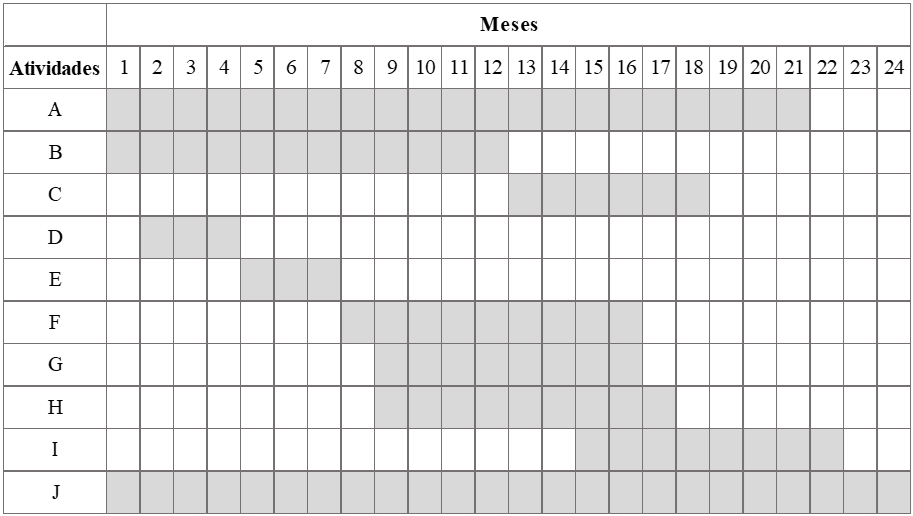
\includegraphics[width=1.0\linewidth]{cronograma.png}
    \caption{Cronograma de atividades}
    {\small Fonte: do Autor, 2025}
    \label{fig51}
\end{figure}




\begin{enumerate}[label=\Alph*.]
    \item{Revisão de Literatura.}  
    
    Pesquisa de trabalhos e bibliografias relacionados ao tema.

    \item{Disciplinas.}  
    
    Cumprimento de disciplinas exigidas pelo programa de mestrado.

    \item{Estágio Docência.}  
    
    Estágio docência em disciplina de graduação.

    \item{Coleta de Dados.}  
    
    Desenvolvimento de algoritmo para realizar a raspagem dos dados (\textit{web scraping}) a partir da base de dados do Fbref.

    \item{Tratamento dos Dados.}  
    
    Desenvolvimento de algoritmos para realizar o tratamento adequado dos dados coletados no item anterior.

    \item{Desenvolvimento dos Modelos Preditivos (ML).}  
    
    Desenvolvimento de modelos preditivos de ML buscando uma previsão razoável de desempenho dos times.

    \item{Experimentos (ML).}  
    
    Teste dos algoritmos obtidos.

    \item{Desenvolvimento da Pesquisa Operacional.}  
    
    Desenvolvimento de modelos de otimização para tarefas no contexto do futebol.

    \item{Experimentos (Pesquisa Operacional).}  
    
    Teste dos modelos obtidos.

    \item{Escrita da Tese.}  
    
    Escrita e apresentação do documento final do trabalho.

\end{enumerate}
